% (c)~2012 Dimitrios Vrettos - d.vrettos@gmail.com
% (c)~2014 Claudio.carboncinii - claudio.carboncini@gmail.com
% (c) 2014 Daniele Zambelli - daniele.zambelli@gmail.com

\chapter{Radicali}

\section{Definizioni}
\label{sec:radici_definizioni}

\subsection{Osservazioni sulle potenze}

\subsubsection{Operazioni inverse}

Quando abbiamo parlato delle operazioni, abbiamo anche accennato all'idea
delle operazioni inverse. Un'operazione inversa è un'operazione che permette
di ``tornare indietro'' rispetto all'effetto prodotto da un'operazione.
Ad esempio se ad un numero qualunque aggiungo~7 e poi tolgo~7 ottengo ancora il 
numero di partenza. Possiamo dire che la sottrazione è l'operazione inversa 
dell'addizione. Così, se parto da un numero~$a$ e lo moltiplico per~$b$ poi lo 
divido per~$b$ ottengo ancora il numero~$a$:

$142 + 7 - 7 = 149 -7 = 142$

$a * b \div b= a$

L'operazione inversa può anche essere vista come quell'operazione he permette 
di trovare un operando conoscendo il risultato:

$\dots + 3 = 7 => \dots = 7 - 3$

$5 + \dots = 9 => \dots = 9 - 5$

$\dots \times 3 = 6 => \dots = 6 \div 3$

$15 \times \dots = 5 => \dots = 15 \div 5$

Le cose si complicano un po' se consideriamo le altre due operazioni 
aritmetiche:

$\dots - 3 = 7 => \dots = 7 \overset{?}{\dots} 3$

$5 - \dots = 9 => \dots = 9 \overset{?}{\dots} 5$

$\dots \div 3 = 6 => \dots = 6 \overset{?}{\dots} 3$

$15 \div \dots = 5 => \dots = 15 \overset{?}{\dots} 5$

Perché Sottrazione e divisione si comportano in modo diverso da addizione e 
moltiplicazione? Come si comporterà la potenza?

Anche la potenza ha due operazioni inverse. Se dobbiamo trovare la base:

$\dots ^3 = 8 \Rightarrow \dots = \sqrt[3]{8} = 2$ (Radice)

mentre per trovare l'esponente:

$2 ^{\dots} = 8 \Rightarrow \dots = \log_{2}{8} = 3$ (Logaritmo)

\begin{definizione}
La \emph{radice} è l'operazione che permette di calcolare la base conoscendo
la potenza e l'esponente.
\end{definizione}

\begin{definizione}
Il \emph{logaritmo} è l'operazione che permette di calcolare l'esponente
conoscendo la potenza e la base.
\end{definizione}

Ne seguito del capitolo ci concentreremo sulle radici rimandando lo studio
dei logaritmi a tempi migliori. 

Iniziamo con alcune definizioni.

\subsection{Radici quadrate}

\begin{definizione}
Si dice \emph{radice quadrata} di un numero reale positivo o nullo quel numero 
reale positivo o nullo che elevato al quadrato dà come risultato il numero dato.
In simboli~$\sqrt a=b \Leftrightarrow b^2=a$ dove $a,b\in \insR^{+} \cup \{0\}$.
\end{definizione}

Il simbolo $\sqrt{\quad}$ è il simbolo della radice quadrata; 
il numero $a$ è detto \emph{radicando}, 
il numero $b$ è detto \emph{radice quadrata} di $a$.

Dalla definizione $\sqrt{a^2}=a$ con $a\ge 0$, quindi: 

$$\sqrt{81}=9 \text{ perché } 9^2=81 \quad 
\sqrt{\frac {9}{64}}=\frac{3}{8}
\text{ perché } \left(\frac 3 8\right)^2=\frac 9{64}$$

\osservazione $\sqrt{81}=\sqrt{(-9)^2}$, ma non è vero che 
$\sqrt{(-9)^2}=-9$ perché nella definizione di radice quadrata abbiamo imposto 
che il risultato dell'operazione di radice quadrata sia sempre un numero 
positivo o nullo.
Questa osservazione ci induce a porre molta attenzione quando il radicando è 
un'espressione letterale: in questo caso $\sqrt{a^2}=a$ non è del tutto 
corretto poiché $a$ può assumere sia valori positivi sia valori negativi
mentre, nei numeri reali, il risultato della radice quadrata non è mai un 
numero negativo. 
Scriveremo correttamente~$\sqrt{a^2}=\valass{a}$.

\begin{exrig}
\begin{esempio}
Radici quadrate
 \begin{multicols}{2}
\begin{itemize}
\item $\sqrt 4=2$ infatti $2^2=4$
\item $\sqrt{\dfrac 9{16}}=\dfrac 3 4$ infatti $\left(\dfrac 3 4\right)^2=
  \dfrac 9{16}$
\item $\sqrt{0,01}=0,1$ infatti $0,1^2=0,01$
\item $\sqrt 1=1$ infatti $1^2=1$
\item $\sqrt 0=0$ infatti $0^2=0$
\item $\sqrt{-16}$ non esiste, radicando negativo;
\item $\sqrt{11}$ esiste ma non è un numero intero né razionale, 
  è un numero irrazionale;
\item $\sqrt{x^2}=\left|x\right|$ dobbiamo mettere il valore assoluto 
  al risultato perché non conoscendo il segno di $x$ dobbiamo imporre che 
  il risultato sia sicuramente positivo;
\item $\sqrt{a^2-4a+4}=\sqrt{(a-2)^2}=\left|a-2\right|$ dobbiamo mettere 
  il valore assoluto perché $a-2$ può anche essere negativo;
\item $\sqrt{9(x+1)^2}=3\left|x+1\right|$.
\end{itemize}
\end{multicols}
\end{esempio}
\end{exrig}

\subsection{Radici cubiche}

\begin{definizione}
 Si dice \emph{radice cubica} di un numero reale $a$ quel numero che, 
 elevato al cubo, dà come risultato $a$. 
 In simboli $\sqrt[3]a=b \Leftrightarrow b^3=a$ dove $a,b\in \insR$.
\end{definizione}

Puoi notare che la radice cubica di un numero reale esiste sempre sia per 
i numeri positivi o nulli, sia per i numeri negativi.

\begin{exrig}
\begin{esempio}
Radici cubiche
 \begin{multicols}{2}
 \begin{itemize}
\item $\sqrt[3]{-8}=-2$ infatti $\left(-2\right)^3=-8$
\item $\sqrt[3]{125}=5$ infatti $5^3=125$
\item $\sqrt[3]1=1$ infatti $1^3=1$
\item $\sqrt[3]0=0$ infatti $0^3=0$
\item $\sqrt[3]{-1000}=-10$ infatti $\left(-10\right)^3=-1000$
\item $\sqrt[3]{\dfrac 1 8}=\dfrac 1 2$ infatti 
  $\left(\dfrac 1 2\right)^3=\dfrac 1 8$
\item $\sqrt[3]{0,125}=0,5$ infatti $(0,5)^3=0,125$
\item $\sqrt[3]{x^3}=x$ per le radici cubiche non si deve mettere 
  il valore assoluto;
\item $\sqrt[3]{x^3+3x^2+3x+1}=\sqrt[3]{(x+1)^3}=x+1$ non si deve mettere 
  il valore assoluto.
\end{itemize}
\end{multicols}
\end{esempio}
\end{exrig}

Osserva che la radice cubica di un numero mantiene sempre lo stesso segno del 
numero in quanto il cubo di un numero reale conserva sempre il segno della 
base.

\subsection{Radici n-esime}
Oltre alle radici quadrate e cubiche si possono considerare radici di indice 
qualsiasi. 
Si parla in generale di radice \emph{n-esima} per indicare una radice con un 
qualsiasi indice $n$.

\begin{definizione}
Si dice \emph{radice n-esima} di un numero reale~$a$ quel numero~$b$ che 
elevato alla~$n$ dà come risultato~$a$. Se~$n$ è pari ~$b$ è positivo.
In simboli~$\sqrt[n]a=b \Leftrightarrow b^n=a$ con $n\in \insN, n > 0$.

$a$ si dice \emph{radicando}, 

$n$ si dice \emph{indice}, 

$b$ si dice \emph{radice}

Non si definisce la radice di indice $0$ e la scrittura $\sqrt[0]a$ è priva 
di significato. Alla scrittura~$\sqrt[1]a$ si dà il valore $a$.
\end{definizione}

Quando si tratta con le radici n-esime di un numero reale, bisogna fare 
attenzione se l'indice della radice è pari o dispari. 
Si presentano infatti i seguenti casi:
\begin{itemize}
 \item se l'indice $n$ è dispari $\sqrt[n]a$ è definita per qualsiasi valore 
  di $a\in \insR$, inoltre è negativa se~$a<0$, positiva se $a>0$ e 
  nulla se $a=0$
 \item se l'indice $n$ è pari $\sqrt[n]a$ è definita solo per i valori 
  di~$a\geq 0$ e si ha che $\sqrt[n]a \ge 0$.
\end{itemize}

\begin{exrig}
\begin{esempio}
Radici n-esime
\begin{multicols}{2}
 \begin{itemize}
 \item $\sqrt[4]{16}=2$ infatti $2^4=16$
 \item $\sqrt[4]{-16}$ non esiste infatti $(-2)^4=+16$
 \item $\sqrt[5]{32}=2$ infatti $2^5=16$
 \item $\sqrt[4]1=1$ infatti $1^4=1$
 \item $\sqrt[n]0=0$
 \item $\sqrt[5]{-1}=-1$ infatti $(-1)^5=-1$
 \item $\sqrt[4]{x^4}=\left|x\right|$ va messo il valore assoluto perché 
   l'indice della radice è pari;
 \item $\sqrt[5]{x^5}=x$ non va messo il valore assoluto perché l'indice 
   della radice è dispari.
\end{itemize}
\end{multicols}
\end{esempio}
\end{exrig}

% \ovalbox{\risolvii \ref{ese:2.1}, \ref{ese:2.2}, \ref{ese:2.3}, \ref{ese:2.4},\ref{ese:2.5}, \ref{ese:2.6},\ref{ese:2.7}, \ref{ese:2.8},\ref{ese:2.9}, \ref{ese:2.10}}

\section{Condizioni di esistenza}
\label{sec:radici_condizioni_esistenza}

Riprendendo le conoscenze sulle potenze, ricordiamo che il quadrato di un 
numero non può essere negativo perché un numero negativo per se stesso dà come 
risultato un numero positivo. 
In generale una potenza con esponente pari è sempre positiva.  
Mentre una potenza con esponente dispari ha lo stesso segno della base.

\begin{esempio}
Alcune potenze:

\begin{multicols}{4}
 $(+5)^2=+25$
 
 $(-5)^2=+25$
 
 $(+2)^6=+64$
 
 $(-2)^6=+64$
 
 $(+2)^3=+8$
 
 $(-2)^3=-8$
 
 $(+2)^7=+128$
 
 $(-2)^7=-128$
\end{multicols}

\end{esempio}

Possiamo affermare che nessun numero reale può essere la radice quadrata di 
un numero negativo, poiché non esiste nessun numero reale che elevato al 
quadrato dia come risultato un numero negativo. 

E, più in generale, nessun numero reale può essere la radice di indice pari 
di un numero negativo.

Finché abbiamo a che fare con numeri, le cose risultano abbastanza semplici, 
ma quando il radicando è un'espressione letterale dobbiamo fare molta 
attenzione a operare su di esso.

Non è detto che $sqrt{a}$ esista, perché non possiamo sapere se~$a$ 
rappresenta un numero positivo o negativo. 
Quindi $sqrt{a}$ è un numero reale solo se~$a \ge 0$.

Le \emph{condizioni di esistenza} (in breve si può scrivere $\CE$) 
di un radicale sono le condizioni cui devono 
soddisfare le variabili che compaiono nel radicando affinché la radice 
sia un numero reale.

Supponiamo di avere $\sqrt[n]{A(x)}$ con $A(x)$ espressione nella
variabile~$x$, dobbiamo distinguere i seguenti casi:
\begin{itemize*}
\item se $n$ è pari la radice è un numero reale solo per i valori 
  di~$x$ che rendono non negativo il radicando, cioè $\CE: A(x)\ge 0$
\item se $n$ è dispari la radice è un numero reale per qualsiasi valore 
  della variabile~$x$ che permette di calcolare il radicando.
\end{itemize*}

\begin{exrig}
\begin{esempio}
Condizioni di esistenza
 \begin{itemize}
 \item $\sqrt x$:\quad $\CE x\ge 0$
 \item $\sqrt[3]x$:\quad $\CE \forall x\in \insR$
 \item $\sqrt{-x}$:\quad $\CE x\le 0$
 \item $\sqrt[3]{-x}$:\quad $\CE \forall x\in \insR$
 \item $\sqrt{x-1}$:\quad $\CE x-1\ge 0 \Rightarrow x\ge 1$
 \item $\sqrt{a^2+1}$:\quad $\CE \forall a\in \insR$, infatti $a^2$ è sempre 
   positivo pertanto $a^2+1>0, \forall a\in \insR$
 \item $\sqrt[3]{\frac 1{x+1}}$:\quad la radice cubica è definita per valori 
   sia positivi sia negativi del radicando, tuttavia bisogna comunque porre la 
   condizione che il denominatore della frazione non sia nullo, 
   quindi $\CE x+1\neq 0 \Rightarrow x\neq -1$
 \item $\sqrt[4]{xy}$:\quad $\CE xy\ge 0$
 \item $\sqrt[5]{a^2(a-3)}$: poiché la radice ha indice dispari non occorre 
   porre alcuna condizione di esistenza.
\end{itemize}
\end{esempio}

\begin{esempio}
 Determina le condizioni di esistenza della seguente 
 espressione: $\sqrt x+\sqrt{x+1}$.

C.E. $\sqrt x$ esiste per $x\ge 0$, $\sqrt{x+1}$ 
esiste per $x+1\ge 0$, quindi per individuare le condizioni di esistenza 
dell'espressione occorre risolvere il sistema 
$\left\{\begin{array}{l} x\ge0\\ x+1\ge0\end{array}\right.
\Rightarrow\left\{\begin{array}{l}x\ge0\\x\ge-1\end{array}\right.$.

\begin{center}
 % (c) 2013 Claudio Carboncini - claudio.carboncini@gmail.com
\begin{tikzpicture}[font=\small,x=10mm, y=10mm]

\draw[->] (0,0) -- (8,0) node [below right] () {$r$};

\foreach \x in {2,5}{
\draw(\x,3pt)--(\x,-3pt);
\begin{scope}[dotted]
\draw (\x,0) -- (\x,-1.5);
\draw (0,-.5) -- (2,-.5);
\draw (0,-1) -- (5,-1);
\end{scope}}

\node[above]  at (2,0) {$-1$};
\node[above]  at (5,0) {$0$};
\pattern[pattern= north east lines, pattern color=red] (5,-1) rectangle (8,-1.5);

\node[below] () at (6.5,-1.5) {$\IS$};

\begin{scope}[blue,thick]
\draw (2,-.5) -- (8,-.5);
\draw (5,-1) -- (8,-1);

\draw[fill=blue] (2,-.5)circle (1.5pt);
\draw[fill=blue] (5,-1)circle (1.5pt);

\end{scope}

\end{tikzpicture}

\end{center}

In definitiva $\CE x\ge 0$.
\end{esempio}

\begin{esempio}
 Determina le condizioni di esistenza della radice 
 $\sqrt[4]{\dfrac{x-1}{x+1}}$.

C.E. $\dfrac{x-1}{x+1}\ge 0$. 
Occorre discutere il segno della frazione $f$, combinando il segno del 
numeratore $N$ e del denominatore $D$:

\begin{center}
 % (c) 2013 Claudio Carboncini - claudio.carboncini@gmail.com
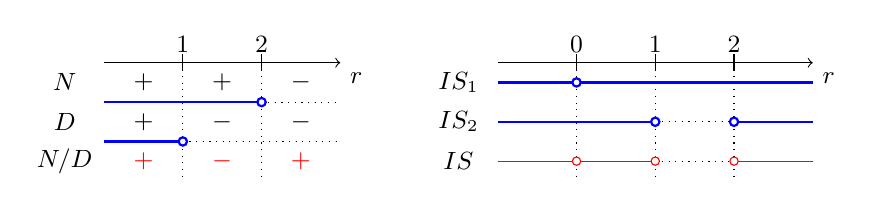
\begin{tikzpicture}[font=\small,x=10mm, y=10mm]

\draw[->] (0,0) -- (3,0) node [below right] () {$r$};
\draw[->] (5,0) -- (9,0) node [below right] () {$r$};

\foreach \x in {1,2,6,7,8}{
\draw(\x,3pt)--(\x,-3pt);
\begin{scope}[dotted]
\draw (\x,0) -- (\x,-1.5);
\draw (2,-.5) -- (3,-.5);
\draw (1,-1) -- (3,-1);
\draw (7,-.75) -- (8,-.75);
\draw (7,-1.25) -- (8,-1.25);
\end{scope}}

\node[above]  at (1,0) {$1$};
\node[above]  at (2,0) {$2$};
\node[above]  at (6,0) {$0$};
\node[above]  at (7,0) {$1$};
\node[above]  at (8,0) {$2$};

\begin{scope}[blue,thick]
\draw (0,-.5) -- (2,-.5);
\draw (1,-1) -- (0,-1);
\draw (5,-.25) -- (6,-.25);
\draw (5,-.25) -- (9,-.25);
\draw (5,-.75) -- (7,-.75);
\draw (8,-.75) -- (9,-.75);

\draw[fill=white] (2,-.5)circle (1.5pt);
\draw[fill=white] (1,-1)circle (1.5pt);
\draw[fill=white] (6,-.25)circle (1.5pt);
\draw[fill=white] (7,-.75)circle (1.5pt);
\draw[fill=white] (8,-.75)circle (1.5pt);
\end{scope}

\foreach \x in {4.5}{
\node  at (\x,-.25) {$IS_1$};
\node  at (\x,-.75) {$IS_2$};
\node  at (\x,-1.25) {$IS$};
}
\foreach \x in {-0.5}{
\node  at (\x,-.25) {$N$};
\node  at (\x,-.75) {$D$};
\node  at (\x,-1.25) {$N/D$};
}

\foreach \z in {.5,1.5}
\node  at (\z,-.25) {$+$};

\foreach \zi in {1.5,2.5}
\node  at (\zi,-.75) {$-$};

\node  at (2.5,-.25) {$-$};
\node  at (0.5,-.75) {$+$};

\begin{scope}[red]
\foreach \y in {-1.25}{
\foreach \ziv in {1.5}
	\node at (\ziv,\y) {$-$};
\foreach \zv in {.5,2.5}
\node at (\zv,\y) {$+$};
\draw (5,-1.25) -- (7,-1.25);
\draw (8,-1.25) -- (9,-1.25);
\draw[fill=white] (6,-1.25)circle (1.5pt);
\draw[fill=white] (7,-1.25)circle (1.5pt);
\draw[fill=white] (8,-1.25)circle (1.5pt);

}
\end{scope}
\end{tikzpicture}

\end{center}
Pertanto C.E. $x<-1\vee x\ge 1$.
\end{esempio}
\end{exrig}

% \vspazio\ovalbox{\risolvii \ref{ese:2.11}, \ref{ese:2.12}, \ref{ese:2.13}, 
% \ref{ese:2.14},\ref{ese:2.15}}

\section{Potenze ad esponente razionale}
\label{sec:radici_esp_razionale}

In questo paragrafo ci proponiamo di scrivere la radice n-esima di un numero 
reale $a\geq0$ sotto forma di potenza di $a$, vogliamo cioè che sia:
$\sqrt[n]a=a^x$.

\paragraph {Caso con esponente positivo}
Elevando ambo i membri dell'uguaglianza alla potenza~$n$ otteniamo: 
$\left(\sqrt[n]a\right)^n=\left(a^x\right)^n$ da cui si ottiene 
$a=a^{n\cdot x}$.
Trattandosi di due potenze con base~$a{\geq}0$, l'uguaglianza è resa possibile 
solo se sono uguali gli esponenti. 
In altre parole, deve essere: $1=n\cdot x \Rightarrow x=\dfrac 1 n$, 
quindi: $\sqrt[n]a=a^{\frac 1 n}$.

Vediamo ora di generalizzare la formula. Sia $m$ un numero intero positivo, 
possiamo scrivere $a^{\frac m n}=\left(a^{\frac 1 n}\right)^m$ e 
quindi $a^{\frac m n}=\left(\sqrt[n]a\right)^m$.

\begin{exrig}
\begin{esempio}
 Calcola le seguenti potenze a esponente razionale positivo.
 \begin{itemize*}
 \item~$27^{\frac 2 3}$: si ha che 
   $27^{\frac 2 3}=\left(\sqrt[3]{27}\right)^2=3^2=9$
 \item~$25^{\frac 3 2}$: si ha che 
   $25^{\frac 3 2}=\left(\sqrt[2]{25}\right)^3=5^3=125$.
\end{itemize*}
\end{esempio}
\end{exrig}

\paragraph{Caso con esponente negativo}
Per definire la potenza ad esponente razionale negativo è necessario imporre 
la restrizione $a{\neq}0$, infatti risulta:
$a^{-\frac m n}=\dfrac 1{a^{\frac m n}}=\left(\dfrac 1 a\right)^{\frac m n}$

\begin{exrig}
\begin{esempio}
 Calcola le seguenti potenze a esponente razionale negativo.
 \begin{itemize*}
 \item $27^{-\frac 2 3}=\dfrac 1{\left(\sqrt[3]{27}\right)^2}=
   \dfrac 1{3^2}=\dfrac 1 9$
 \item $125^{-\frac 2 3}=\sqrt[3]{125^{-2}}=\sqrt[3]{(5^3)^{-2}}=
   \sqrt[3]{(5^{-2})^3}=5^{-2}=\dfrac 1{25}$
 \item $\left(\dfrac 1 8\right)^{-\frac 3 2}=
   \sqrt{\left(\dfrac 1 8\right)^{-3}}=\sqrt{8^3}=\sqrt{(2^3)^3}=\sqrt{2^9}$
 \item $\left(\dfrac 1{49}\right)^{-\frac 1 2}=(49)^{\frac 1 2}=\sqrt{49}=7$
\end{itemize*}
\end{esempio}
\end{exrig}

In generale si dà la seguente
\begin{definizione}
Si dice \emph{potenza a esponente razionale} $\frac m n$ di un numero reale 
positivo $a$ l'espressione:
 $a^{\frac m n}=\sqrt[n]{a^m}=\left(\sqrt[n]a\right)^m$ con 
 $\frac m n\in \insQ$.
\end{definizione}

Perché abbiamo dovuto imporre la condizione che~$a$ sia un numero positivo?
Partiamo dall'espressione $a^{\frac 1 n}$ con $n\in \insN-\{0\}$, 
se $n$ è dispari la potenza $a^{\frac 1 n}$ è sempre definita per ogni valore 
della base $a$, mentre se è pari $a^{\frac 1 n}$ è definita solo 
per $a{\geq}0$.

Nel caso generale $a^{\frac m n}$ con $\frac m n\in \insQ$ 
la formula $a^{\frac m n}=\left(\sqrt[n]a\right)^m$ è falsa se $a<0$.

Consideriamo il seguente esempio:
$(-2)^{\frac 6 6}=\left[(-2)^{\frac 1 6}\right]^6=\left(\sqrt[6]{-2}\right)^6$ 
non è definita nei numeri reali perché non esiste la radice sesta di un numero 
negativo.
Tuttavia possiamo anche scrivere 

\[(-2)^{\frac 6 6}=\left[(-2)^6\right]^{\frac 1 6}=(64)^{\frac 1 6}=
\sqrt[6]{64}=2.\]

Arriviamo pertanto a due risultati differenti.

Per estendere la definizione al caso di basi negative sarebbe necessario 
stabilire un ordine di priorità delle operazioni ma ciò andrebbe contro la 
proprietà commutativa del prodotto degli esponenti di una potenza di potenza.

% \vspazio\ovalbox{\risolvii \ref{ese:2.16}, \ref{ese:2.17}, \ref{ese:2.18}, 
% \ref{ese:2.19},\ref{ese:2.20}}

\section{Semplificazione di radici}
\label{sec:radici_semplificazione}

\begin{proposizione}
Il valore di una radice in $\insR^+\cup \{0\}$ non cambia se moltiplichiamo 
o dividiamo l'indice della radice e l'esponente del radicando per uno stesso 
numero positivo. 
In simboli 
\[\sqrt[n]{a^m}=a^{\frac{m}{n}}=a^{\frac{mt}{nt}}=\sqrt[nt]{a^{mt}}\]
con $a\ge 0$ e $m,n,t\in \insN-\{0\}$.
\end{proposizione}

% \newpage
% \begin{exrig}
%  \begin{esempio}
%  Radici equivalenti.
%  \begin{itemize}
%  \item $\sqrt 2=\sqrt[4]{2^2}$ abbiamo moltiplicato per $2$ indice della 
%   radice ed esponente del radicando;
%  \item $\sqrt[3]a=\sqrt[9]{a^3}$ abbiamo moltiplicato per $3$ indice della 
%   radice ed esponente del radicando.
% \end{itemize}
%  \end{esempio}
% \end{exrig}
% 
% \begin{proposizione}
% Il valore di una radice in $\insR^+\cup \{0\}$ non cambia se dividiamo 
% l'indice della radice e l'esponente del radicando per un loro divisore comune. 
% In simboli $\sqrt[nt]{a^{mt}}=\sqrt[n]{a^m}$ con $a\ge 0$ e 
% $m,n,t\in \insN-\{0\}$.
% \end{proposizione}

\begin{exrig}
 \begin{esempio}
Semplificazione di radici
\begin{itemize}
 \item $\sqrt[4]{5^2}=5^{\frac{2}{4}}=5^{\frac{1}{2}}=\sqrt 5$: 
  abbiamo semplificato per $2$ indice della radice ed esponente del radicando;
 \item $\sqrt[4]{(-3)^2}=\sqrt[4]{3^2}=3^{\frac{2}{4}}=3^{\frac{1}{2}}=\sqrt 3$
 \item $\sqrt[10]{4^{15}}=4^{\frac{15}{10}}=4^{\frac{3}{2}}=\sqrt{4^3}$: 
  abbiamo semplificato per $5$
 \item $\sqrt[7]{3^9}=3^{\frac{9}{7}}$: 
  non è riducibile perché indice della radice ed esponente non hanno divisori 
  comuni;
 \item $\sqrt[8]{2^6}=2^{\frac{6}{8}}=2^{\frac{3}{4}}=\sqrt[4]{2^3}$
 \item $\sqrt[6]{\left(\dfrac{1}{5}\right)^{-9}}=\sqrt[6]{5^9}=
        5^{\frac{9}{6}}=5^{\frac{3}{2}}=\sqrt[2]{5^3}$
 \item $\sqrt{10^{-4}}=10^{-\frac{4}{2}}=10^{-2}=\frac 1{100}$
 \item $\sqrt{30\cdot 27\cdot 10}$: scomponendo in fattori primi otteniamo 
  \[\sqrt{30\cdot 27\cdot 10}=
    \sqrt{2\cdot 3\cdot 5\cdot 3^3\cdot 2\cdot 5}=
    \sqrt{2^2\cdot 3^4\cdot 5^2}.\] 
    Osserviamo che tutti gli esponenti del radicando e l'indice della radice 
    hanno un divisore, quindi 
    $\sqrt{2^2\cdot 3^4\cdot 5^2}=
     2^{\frac{2}{2}} \cdot 3^{\frac{4}{2}} \cdot 5^{\frac{2}{2}}=
     2\cdot 3^2\cdot 5=90$
\end{itemize}
\end{esempio}
\end{exrig}

Fin'ora abbiamo operato con numeri, ma se il radicando è un'espressione 
letterale non sappiamo se sia positiva o negativa e quando semplifichiamo un 
esponente pari dobbiamo tenerne conto:

\begin{esempio}
 Se abbiamo la radice:~$\sqrt[4]{a^2}$ potremmo pensare di semplificarla in:
 
 \[\sqrt[4]{a^2}=a^{\frac{2}{4}}=a^{\frac{1}{2}}=\sqrt a\]
 
 Ora, se $a=+5$ ci ritroviamo esattamente come nel primo degli esempi 
 precedenti. Se $a=-5$ lo svolgimento precedente ci darebbe: $\sqrt {-5}$ 
 che non è un numero reale perché la radice ha indice pari e il radicando 
 è negativo, mentre l'espressione iniziale equivale ad un numero reale dato 
 che il radicando, essendo elevato alla seconda è senz'altro positivo.
 Possiamo risolvere questo errore utilizzando il valore assoluto.
\end{esempio}

Nel caso di radicandi letterali la regola della semplificazione delle radici 
diventa:

\begin{proposizione}
 \[\sqrt[nt]{a^{mt}}=\left\{\begin{array}{l}
   \sqrt[n]{a^m} \text{ se }t \text{ è dispari}\\
   \sqrt[n]{\left|a^m\right|}\text{, se }t\text{ è pari}
 \end{array}\right.\]
\end{proposizione}

\begin{exrig}
 \begin{esempio}
Semplificazione di radici con espressione letterale come radicando.
\begin{itemize}
\item $\sqrt{4x^4y^2a^6}=\sqrt{2^2x^4y^2a^6}=2x^2\left|ya^3\right|$: 
 abbiamo semplificato per $2$ sia l'indice della radice che l'esponente del 
 radicando;
\item $\sqrt[12]{a^2+2a+1}=\sqrt[12]{(a+1)^2}=\sqrt[6]{\left|a+1\right|}$: 
 dopo aver riconosciuto che il radicando è il quadrato del binomio, 
 abbiamo semplificato per $2$ indice ed esponente;
\item $\sqrt{x^2y^2}=\valass{xy}$
\item $\sqrt{x^2+2xy+y^2}=\sqrt{(x+y)^2}=\valass{x+y}$
\item $\sqrt{x^2+y^2}$ non è semplificabile perché il radicando non può essere 
 espresso sotto forma di potenza;
\item $\sqrt[6]{(x-1)^2}=\sqrt[3]{\valass{x-1}}$
\end{itemize}
 \end{esempio}
\end{exrig}

% La proprietà invariantiva si può applicare per semplificare i radicali se la 
% base del radicando è positiva o nulla, se fosse negativa si potrebbe perdere 
% la concordanza del segno. 
% Per esempio~$\sqrt[10]{(-2)^6}\neq \sqrt[5]{(-2)^3}$, infatti il primo 
% radicando è positivo mentre il secondo è negativo.
% 
% Invece $\sqrt[9]{(-2)^3}=\sqrt[3]{-2}$ perché in questo caso la concordanza 
% del segno è conservata, infatti pur essendo la base negativa, l'esponente 
% resta dispari, conservando il segno della base.
% 
% Se il radicando ha base negativa e nella semplificazione il suo esponente 
% passa da pari a dispari è necessario mettere il radicando in valore assoluto: 
% $\sqrt[10]{(-2)^6}=\sqrt[5]{\left|-2^3\right|}$.
% 
% Se il radicando è letterale si segue la stessa procedura: ogni volta che 
% studiando il segno del radicando si trova che la base può essere negativa, 
% se l'esponente del radicando passa da pari a dispari, si mette il modulo per 
% garantire la concordanza del segno:
% $\sqrt[10]{x^6}=\sqrt[5]{\left|x^3\right|}$, $\CE \forall x \in \insR$.

% \vspazio\ovalbox{\risolvii \ref{ese:2.21}, \ref{ese:2.22}, \ref{ese:2.23}, \ref{ese:2.24},\ref{ese:2.25},\ref{ese:2.26},\ref{ese:2.27},\ref{ese:2.28},\ref{ese:2.29},\ref{ese:2.30},\ref{ese:2.31}}

\section{Moltiplicazione e divisione di radici}
\label{sec:radici_moltiplicazione}

Se abbiamo radicali letterali, prima di operare, è necessario determinare le 
condizioni di esistenza: il prodotto di due radicali esiste là dove sono 
soddisfatte le condizioni di esistenza di tutti i fattori; 
il quoziente esiste là dove sono soddisfatte le condizioni di esistenza di 
dividendo e divisore, con il divisore diverso da zero.

Una volta verificate le condizioni di esistenza, possiamo trasformare le
radici in potenze con esponente frazionario, operare su queste espressioni 
utilizzando le proprietà delle potenze e ritrasformare il risultato in radici.

\begin{exrig}
 \begin{esempio}
Moltiplicazione e divisione di radici con lo stesso radicando.
\begin{itemize}
\item $\sqrt[4]6\cdot \sqrt[3]6=6^{\frac 1 4}\cdot 6^{\frac 1 3}=
       6^{\frac 1 4+\frac 1 3}=6^{\frac 7{12}}=\sqrt[12]{6^7}$
\item $\sqrt[4]6:\sqrt[3]6=6^{\frac 1 4}:6^{\frac 1 3}=
       6^{\frac 1 4-\frac 1 3}=6^{-\frac 1{12}}=\frac 1{\sqrt[12]6}$.
\end{itemize}
 \end{esempio}
\end{exrig}

\subsection{Moltiplicazione e divisione di radici con lo stesso indice}
Il prodotto di due radici che hanno lo stesso indice è una radice che ha per 
indice lo stesso indice e per radicando il prodotto dei radicandi:
\[\sqrt[n]a\cdot \sqrt[n]b=\sqrt[n]{ab}.\]

Allo stesso modo, il quoziente di due radici che hanno lo stesso indice è una 
radice che ha per indice lo stesso indice e \ per radicando il quoziente dei 
radicandi:
\[\sqrt[n]a:\sqrt[n]b=\sqrt[n]{a:b} \Rightarrow \dfrac{\sqrt[n]a}{\sqrt[n]b}=
  \sqrt[n]{\dfrac a b}.\]

\emph{Nota}: 
 Se $a$ e $b$ sono entrambi negativi e l'indice è pari, l'espressione
 $\sqrt[n]a:\sqrt[n]b$ non ha valori reali mentre $\sqrt[n]{ab}$ ha il
 radicando positivo e quindi ha valori reali. Moltiplicando in questo modo 
 possiamo ottenere un risultato reale che l'espressione di partenza non ha.

Per rendersi conto di questa proprietà si possono trasformare le radici in 
potenze ad esponenti razionali e applicare le proprietà delle potenze:
 \[\sqrt[n]a\cdot \sqrt[n]b=a^{\frac 1 n}\cdot b^{\frac 1 n}=(ab)^{\frac 1 n}=
   \sqrt[n]{ab},\quad \sqrt[n]a:\sqrt[n]b=a^{\frac 1 n}:b^{\frac 1 n}=
   \left(\dfrac a b\right)^{\frac 1 n}=\sqrt[n]{\dfrac a b}.\]

\begin{exrig}
 \begin{esempio}
Moltiplicazione e divisione di radici con lo stesso indice.
\begin{itemize}
\item $\sqrt{2} \cdot \sqrt{3}=\sqrt{2 \cdot 3}=\sqrt 6$
\item $\sqrt{2} \cdot \sqrt{3}=
       2^{\frac{1}{2}} \cdot 3^{\frac{1}{2}}=(2  \cdot 3)^{\frac{1}{2}}=
       6^{\frac{1}{2}}=\sqrt 6$
\item $\frac{\sqrt[3]9}{\sqrt[3]{72}}=\sqrt[3]{\frac 9{72}}=
       \sqrt[3]{\frac 1 8}=\frac 1 2$
\item $\sqrt{2a}\cdot \sqrt{\frac a b}:\sqrt{\frac {2b} 9}=
       \sqrt{2a}\cdot \sqrt{\frac a b}:\sqrt{\frac {2b} 9}=
       \sqrt{2a\cdot \frac a b\cdot \frac 9{2b}}=\sqrt{\frac{9a^2}{b^2}}=
       \frac {3a} b 
      (\CE a\ge 0\wedge b>0)$.
\end{itemize}
 \end{esempio}
\end{exrig}

\subsection{Moltiplicazione e divisione di radici con indici diversi}

\begin{procedura}
Moltiplicazione o divisione di radici generiche:
\begin{enumeratea}
 \item scomporre in fattori irriducibili tutti i radicandi;
 \item porre le condizioni di esistenza;
 \item scrivere le radici sotto forma di potenza;
 \item applicare le proprietà delle potenze.
\end{enumeratea}
\end{procedura}

\begin{exrig}
 \begin{esempio}
Moltiplicazione e divisione di radici con indice diverso.
\begin{itemize}
\item $\sqrt 2\cdot \sqrt[3]2=
       2^\frac{1}{2} \cdot 2^\frac{1}{3} = 2^{\frac{1}{2} + \frac{1}{3}} =
       2^{\frac{3+2}{6}} = 2^{\frac{5}{6}} =\sqrt[6]{2^5}$
\item 
  $\sqrt[3]{\frac{3}{2}} \cdot \sqrt[4]{\frac{8}{27}} : \sqrt[6]{\frac{2}{3}}=
   \left(\frac{3}{2}\right)^{\frac{1}{3}} \cdot 
   \left(\frac{2^3}{3^3}\right)^{\frac{1}{4}} : 
   \left(\frac{2}{3}\right)^{\frac{1}{6}}=
   \left(\frac{3}{2}\right)^{\frac{4}{12}} \cdot 
   \left(\frac{2^3}{3^3}\right)^{\frac{3}{12}} : 
   \left(\frac{2}{3}\right)^{\frac{2}{12}}=
   \left(\frac{3^4}{2^4} \cdot 
   \frac{2^9}{3^9} \cdot 
   \frac{3^2}{2^2}\right)^{\frac{1}{12}}=
   \left(\frac{2^3}{3^3}\right)^{\frac{1}{12}}=
   \left(\frac{2}{3}\right)^{\frac{3}{12}}=
   \left(\frac{2}{3}\right)^{\frac{1}{4}}=\sqrt[4]{\frac 2 3}$
\end{itemize}
 \end{esempio}

\begin{esempio}
Prodotto di radici con radicandi letterali.
 $\dfrac{\sqrt[3]{x^2y}\cdot \sqrt{xy}}{\sqrt[6]{x^2y^3}}$
 
 Il campo di esistenza è: $\CE x>0\wedge y>0$.
 
\begin{align*}
\dfrac{\sqrt[3]{x^2y}\cdot \sqrt{xy}}{\sqrt[6]{x^2y^3}} &=
\frac{{x^\frac{2}{3} \cdot y^\frac{1}{3}} \cdot 
       x^\frac{1}{2} \cdot y^\frac{1}{2}}
     {x^\frac{2}{6} \cdot y^\frac{3}{6}} =
         & \mbox{scrittura sotto forma di potenze}\\
    &=x^\frac{2}{3} \cdot x^\frac{1}{2} : x^\frac{2}{6} \cdot 
      y^\frac{1}{3} \cdot y^\frac{1}{2} : y^\frac{3}{6}=
         & \mbox{proprietà commutativa} \\
    &=x^{\frac{2}{3} + \frac{1}{2} - \frac{2}{6}} \cdot 
      y^{\frac{1}{3} + \frac{1}{2} - \frac{3}{6}}= 
         & \mbox{proprietà delle potenze}\\
    &=x^{\frac{4+3-2}{6}} \cdot y^{\frac{2+3-3}{6}}=
         & \mbox{calcolo degli esponenti} \\
    &=x^{\frac{5}{6}} \cdot y^{\frac{2}{6}}=
    \sqrt[6]{x^5y^2}
\end{align*}

% \[\frac{\sqrt[3]{x^2y}\cdot \sqrt{\mathit{xy}}}{\sqrt[6]{x^2y^3}}=
%         \sqrt[6]{\frac{\left(x^2y\right)^2\cdot (xy)^3}{x^2y^3}}=
%         \sqrt[6]{\frac{x^4y^2x^3y^3}{x^2y^3}}=
%         \sqrt[6]{\frac{x^7y^5}{x^2y^3}}=
%         \sqrt[6]{x^5y^2}.
% \]
\end{esempio}

% \begin{esempio}
%  $\sqrt[3]{\dfrac{ax+a}{x^2+2x+1}}\cdot \sqrt{\dfrac{x^2-2x+1}{ax-a}}$
%  
% \begin{enumeratea}
% \item Scomponiamo in fattori i radicandi 
%  $\sqrt[3]{\dfrac{a(x+1)}{(x+1)^2}}\cdot \sqrt{\dfrac{(x-1)^2}{a(x-1)}}$
% \item $\CE$\, $x+1\neq 0\wedge a(x-1)>0\Rightarrow x\neq -1\wedge 
%  ((a>0\wedge x>1)\vee (a<0\wedge x<1))$
% \item Semplifichiamo le frazioni di ciascun radicando 
%  $\sqrt[3]{\dfrac a{x+1}}\cdot \sqrt{\dfrac{x-1} a}$
% \item Trasformiamo nello stesso indice: il~$\mcm$ degli indici è~$6$, quindi:
% \[
% \sqrt[6]{\left(\dfrac a{x+1}\right)^2}\cdot 
% \sqrt[6]{\left(\dfrac{x-1} a\right)^3}=
%  \sqrt[6]{\dfrac{a^2}{(x+1)^2}\cdot \dfrac{(x-1)^3}{a^3}}=
%  \sqrt[6]{\dfrac{(x-1)^3}{a(x+1)^2}}
% \]
% \end{enumeratea}
% \end{esempio}
% 
% \begin{esempio}
%  $\sqrt[3]{\dfrac{x^2}{x^2-2x+1}}:\sqrt[4]{\dfrac{x^4-2x^2+1}{x^2-1}}$.
% 
%  \begin{enumeratea}
% \item Scomponiamo in fattori i radicandi
%  $\sqrt[3]{\dfrac{x^2}{(x-1)^2}}:
%  \sqrt[4]{\dfrac{(x-1)^2\cdot (x+1)^2}{(x+1)(x-1)}}$
% \item $\CE$\, $(x-1)(x+1)>0\Rightarrow x<-1\vee x>1$. 
%  L'operazione che dobbiamo eseguire è una divisione e dunque il divisore deve 
%  essere diverso da zero, quindi $x\neq -1\wedge x\neq 1$, comunque già 
%  implicite nelle C.E. trovate;
%  
% \begin{center}
%  % (c) 2013 Claudio Carboncini - claudio.carboncini@gmail.com
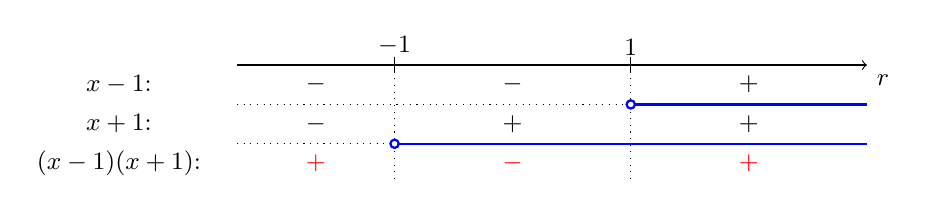
\begin{tikzpicture}[font=\small,x=10mm, y=10mm]

\draw[->] (0,0) -- (8,0) node [below right] () {$r$};

\foreach \x in {2,5}{
\draw(\x,3pt)--(\x,-3pt);
\begin{scope}[dotted]
\draw (\x,0) -- (\x,-1.5);
\draw (0,-.5) -- (5,-.5);
\draw (0,-1) -- (2,-1);
\end{scope}}

\node[above]  at (2,0) {$-1$};
\node[above]  at (5,0) {$1$};

\begin{scope}[blue,thick]
\draw (5,-.5) -- (8,-.5);
\draw (2,-1) -- (8,-1);

\draw[fill=white] (5,-.5)circle (1.5pt);
\draw[fill=white] (2,-1)circle (1.5pt);
\end{scope}

\foreach \x in {-1.5}{
\node  at (\x,-.25) {$x-1$:};
\node  at (\x,-.75) {$x+1$:};
\node  at (\x,-1.25) {$(x-1)(x+1)$:};
}
\foreach \z in {1,3.5}{
\node  at (\z,-.25) {$-$};
}
\foreach \zi in {3.5, 6.5}{
\node  at (\zi,-.75) {$+$};
}

\node  at (6.5,-.25) {$+$};
\node  at (1,-.75) {$-$};

\begin{scope}[red]
\foreach \zii in {1, 6.5}{
\node  at (\zii,-1.25) {$+$};
}
\node  at (3.5,-1.25) {$-$};
\end{scope}
\end{tikzpicture}

% \end{center}
% \item Semplifichiamo i radicandi 
%  $\sqrt[3]{\dfrac{x^2}{(x-1)^2}}:\sqrt[4]{(x-1)\cdot (x+1)}$
% \item Riduciamo allo stesso indice: il $\mcm$ degli indici è $12$, quindi:
% 
% $\sqrt[12]{\left[\frac{x^2}{(x-1)^2}\right]^4}:\sqrt[12]{(x-1)^3 (x+1)^3}
% \Rightarrow 
% \sqrt[12]{\frac{x^8}{(x-1)^8}\cdot \frac 1{(x-1)^3 (x+1)^3}}=
% \sqrt[12]{\frac{x^8}{(x-1)^{11}(x+1)^3}}$.
% \end{enumeratea}
% \end{esempio}
\end{exrig}

% \vspazio\ovalbox{\risolvii \ref{ese:2.32}, \ref{ese:2.33}, \ref{ese:2.34}, 
% \ref{ese:2.35},\ref{ese:2.36},\ref{ese:2.37},\ref{ese:2.38},\ref{ese:2.39}}

\section{Portare un fattore sotto il segno di radice}
\label{sec:radici_portare_dentro}

Per portare un fattore dentro il segno di radice bisogna elevarlo all'indice 
della radice:
\begin{itemize*}
 \item $a\sqrt[n]b=\sqrt[n]{a^n\cdot b}$ se $n$ è pari e $a\ge 0$
 \item $a\sqrt[n]b=-\sqrt[n]{a^n\cdot b}$ se $n$ è pari e $a<0$
 \item $a\sqrt[n]b=\sqrt[n]{a^n\cdot b}$ se $n$ è dispari.
\end{itemize*}

Ricordando che abbiamo posto $\sqrt[1]a=a$, portare un fattore sotto radice 
equivale a svolgere la moltiplicazione tra una radice di indice $1$ e una 
radice di indice qualsiasi.
\begin{exrig}
 \begin{esempio}
 Portare un numero reale dentro il segno di radice.
 \begin{itemize}
 \item $2\cdot \sqrt[3]7=\sqrt[3]{2^3\cdot 7}=\sqrt[3]{56}$
 \item $3\cdot \sqrt{\frac 2{21}}=\sqrt{3^2\cdot \frac 2{21}}=
        \sqrt{9\cdot \frac 2{21}}=\sqrt{\frac 6 7}$
 \item $-\frac 1 2\sqrt 3$\, lasciamo fuori dalla radice il segno meno 
       $-\frac 1 2\sqrt 3=-\sqrt{\left(\frac 1 2\right)^2\cdot 3}=
        -\sqrt{\frac 3 4}$
 \item $-\frac 1 3\cdot \sqrt{12}=-\sqrt{\left(\frac 1 3\right)^2\cdot 12}=
        -\sqrt{\frac 1 9\cdot 12}=-\sqrt{\frac 4 3}$
 \item $(1-\sqrt 2)\cdot \sqrt 3=-(\sqrt 2-1)\cdot \sqrt 3=
        -\sqrt{(\sqrt 2-1)^2\cdot 3}$
 \item $-2\sqrt[3]5=\sqrt[3]{(-2)^3\cdot 5}=\sqrt[3]{-40}$.
 \end{itemize}
 \end{esempio}

 \begin{esempio}
 Portare una espressione letterale dentro il segno di radice.
 \begin{itemize}
 \item $a\cdot \sqrt[3]b=\sqrt[3]{a^3b}$\, l'indice della radice è dispari 
  pertanto si porta sotto radice senza alcuna condizione;
 \item $(x-1)\cdot \sqrt[3]x=\sqrt[3]{(x-1)^3\cdot x}$\, l'indice della radice 
  è dispari, non sono necessarie condizioni sulla $x$
 \item $(x-2)\sqrt y$\, osserviamo che il radicale esiste per $y\ge 0$.
  Per portare dentro il segno di radice il coefficiente $(x-2)$ bisogna fare 
  la distinzione:
 \[
 (x-2)\sqrt y=\left\{\begin{array}{l}\sqrt{(x-2)^2y}\text{, se }x\ge 2\\
 -(2-x)\sqrt y=-\sqrt{(2-x)^2y}\text{, se }x<2;\end{array}\right.
 \]
 \item $(x-1)\sqrt{x-2}$.\, Il radicale esiste per $x-2\ge 0\ \to \ x\ge 2$, 
 per questi valori il coefficiente esterno $(x-1)$ è positivo e può essere 
 portato dentro la radice: \[(x-1)\sqrt{x-2}=\sqrt{(x-1)^2(x-2)};\]
%  \item $\frac{a-1}{a+3}\cdot \sqrt{\frac{a+2}{(a-1)^2}}$. Determiniamo le 
%  condizioni di esistenza del radicale: per l'esistenza della frazione 
%  $\frac{a+2}{(a-1)^2}$ deve essere $(a-1)^2\neq 0$, ovvero $a\neq 1$. 
%  Affinché il radicando sia positivo o nullo, essendo il denominatore sempre 
%  positivo (ovviamente per $a\neq 1$) è sufficiente che sia $a+2\geqslant 0$ 
%  ovvero $a\geqslant -2$. 
%  Pertanto le condizioni di esistenza sono~ $a\geqslant -2$ e $a\neq 1$.
% 
%  Studiamo ora il segno della frazione algebrica da portare sotto radice: 
%  tale frazione è positiva o nulla per $a<-3\vee a\geqslant 1$, è negativa 
%  per $-3<a\leqslant 1$.
% 
%  Se $a>1$ si ha 
%  $\frac{a-1}{a+3}\cdot \sqrt{\frac{a+2}{(a-1)^2}}=
%   \sqrt{\frac{(a-1)^2}{(a+3)^2}\cdot \frac{a+2}{(a-1)^2}}=
%   \sqrt{\frac{a+2}{(a+3)^2}}$.
% 
%  Se $-2<a<1$ il fattore da portare sotto radice è negativo, quindi:
%  \[-\left(-\frac{a-1}{a+3}\right)\cdot \sqrt{\frac{a+2}{(a-1)^2}}=
%    -\sqrt{\frac{[-(a-1)]^2}{(a+3)^2}\cdot \frac{a+2}{(a-1)^2}}=
%    -\sqrt{\frac{a+2}{(a+3)^2}}\]
% 
%  Se $a=-2$ l'espressione da calcolare vale zero mentre il caso $a=1$ è escluso 
%  dalla condizione di esistenza.
 \end{itemize}
 \end{esempio}
\end{exrig}
% \vspazio\ovalbox{\risolvii \ref{ese:2.40}, \ref{ese:2.41}}

\section{Portare un fattore fuori dal segno di radice}
\label{sec:radici_portare_fuori}

È possibile portare fuori dal segno di radice quei fattori aventi come 
esponente un numero che sia maggiore o uguale all'indice della radice. 
In generale si inizia scomponendo in fattori irriducibili il radicando, 
ottenendo un radicale del tipo $\sqrt[n]{a^m}$ con $m\ge n$.

\paragraph{I° modo:} si esegue la divisione intera $m:n$ ottenendo un 
quoziente $q$ e un resto $r$. Per la proprietà della divisione si 
ha $m=n\cdot q+r$ quindi $\sqrt[n]{a^m}=\sqrt[n]{a^{n\cdot q+r}}$ 
e per le proprietà delle potenze 
$\sqrt[n]{a^{n\cdot q+r}}=\sqrt[n]{(a^q)^n\cdot a^r}$ 
e per la regola del prodotto di due radici con medesimo indice si ottiene:

\[\sqrt[n]{a^{n\cdot q+r}}= \sqrt[n]{(a^q)^n\cdot a^r}=
  \sqrt[n]{(a^q)^n}\cdot \sqrt[n]{a^r}=
  a^q\cdot \sqrt[n]{a^r}\text{ con } r<n.\]
Notiamo che il fattore ``fuori`` dalla radice ha per esponente il quoziente 
della divisione intera, mentre il fattore che rimane ``dentro`` ha per 
esponente il resto della divisione stessa.

 $\sqrt[3]{a^8}=\ldots $ eseguiamo la divisione $8:3$ con $q=2$ e $r=2$, 
 otteniamo $\sqrt[3]{a^8}=a^2\cdot \sqrt[3]{a^2}$.

\paragraph{II° modo:} si può trasformare la potenza del radicando nel 
prodotto di due potenze con la stessa base; una avente esponente multiplo 
dell'indice della radice e l'altra avente per esponente la differenza tra 
l'esponente iniziale e il multiplo trovato. Consideriamo il seguente esempio:

 $\sqrt[3]{a^8}=\ldots $ il multiplo di $3$ più vicino a $8$ è $6$ quindi, 
 otteniamo 
\[\sqrt[3]{a^8}=\sqrt[3]{a^6\cdot a^2}=\sqrt[3]{a^6}\cdot \sqrt[3]{a^2}=
  a^2\cdot \sqrt[3]{a^2}.\]

\begin{exrig}
 \begin{esempio}
 Portare un numero reale fuori dal segno di radice.
\begin{itemize}
 \item $\sqrt{1200}$ Si scompone in fattori primi il radicando 
       $1200=2^4\cdot 5^2\cdot 3$ ne segue allora che 
       $\sqrt{1200}=\sqrt{2^4\cdot 5^2\cdot 3}=2^2\cdot 5\sqrt 3=20\sqrt 3$
 \item $\sqrt{75}=\sqrt{5^2\cdot 3}=5\sqrt 3$
 \item $\sqrt{720}=\sqrt{2^4\cdot 3^2\cdot 5}=
        2^2\cdot 3\cdot \sqrt 5=12\sqrt 5$
\end{itemize}
 \end{esempio}
\end{exrig}

Quando portiamo fuori dalla radice un termine letterale dobbiamo verificare 
se l'indice della radice è pari o dispari e se il termine che portiamo fuori 
è positivo o negativo. In particolare:
\[\sqrt[n]{a^nb}=\left\{\begin{array}{l}
 a\sqrt[n]b\text{, se }n\text{ dispari;}\\
 \valass a\sqrt[n]b\text{, se }n\text{ pari.}\end{array}\right.\]

\begin{exrig}
 \begin{esempio}
 Portare una espressione letterale fuori dal segno di radice.
\begin{itemize}
 \item $\sqrt{2a^2}=\valass a\sqrt 2$ bisogna mettere $a$ in valore assoluto 
 perché sotto radice poteva essere sia negativo che positivo, la radice invece 
 deve essere sempre positiva; se $a<0$ la relazione~$\sqrt{2a^2}=a\sqrt 2$ è 
 errata;
 \item $\sqrt[3]{a^5b^7cd^3}$ occorre eseguire le divisioni intere tra gli 
 esponenti e l'indice della radice. Cominciamo da $a^5$ risulta $5:3 = 1$ con 
 resto uguale a $2$ per $b^7$ si ha $7:3$ con quoziente~$2$ e resto~$1$ 
 l'esponente di $c$ è minore dell'indice; per $d^3$ si ha $3:3$ con quoziente 
 $1$ e resto~$0$. In definitiva 
 $\sqrt[3]{a^5b^7cd^3}={ab}^2 d\sqrt[3]{a^2{bc}}$, o anche:
 
\[\sqrt[3]{a^5b^7cd^3}=\sqrt[3]{(a^3a^2)(b^6b)cd^3}=
  \sqrt[3]{a^3b^6d^3}\cdot \sqrt[3]{a^2bc}=ab^2d^3\sqrt[3]{a^2bc}\]
  
In questo caso non c'è da mettere il valore assoluto perché l'indice della 
radice è dispari;
 \item $\sqrt[3]{\dfrac{3^3x^3y}{z^6}}$,\, 
       $\CE z\neq 0\,\sqrt[3]{\dfrac{3^3x^3y}{z^6}}=3\dfrac x{z^2}\sqrt[3]y$
%  \item$\sqrt[4]{4x^4-4x^5}$ 
%   scomponiamo il radicando per poter studiare le condizioni di esistenza del 
%   radicale e portare fuori qualche fattore: 
%   \[\sqrt[4]{4x^4-4x^5}=\sqrt[4]{4x^4(1-x)} \CE 1-x\ge 0\Rightarrow \ x\le 1.\]
%   Pertanto:
%   \[\sqrt[4]{4x^4-4x^5}=\sqrt[4]{4x^4(1-x)}=\valass x\sqrt[4]{4(1-x)}=
%     \left\{\begin{array}{l}
%     x\sqrt[4]{4(1-x)}\text{, se }0\le x\le 1\\
%     -x\sqrt[4]{4(1-x)}\text{, se }x<0.\end{array};\right.\]
 \item $\sqrt{3(a-1)^2}=\valass{a-1}\sqrt 3=\left\{\begin{array}{l}
   -(a-1)\sqrt 3\text{, se }a < 1 \\
   (a-1)\sqrt 3\text{, se }a \ge 1
 .\end{array}\right.$.
\end{itemize}
 \end{esempio}
\end{exrig}
% \vspazio\ovalbox{\risolvii \ref{ese:2.42}, \ref{ese:2.43}, \ref{ese:2.44}, \ref{ese:2.45}}

\section{Potenza di radice e radice di radice}
\label{sec:radici_potenza}

Per elevare a potenza una radice si eleva a quella potenza il radicando: 
$\left(\sqrt[n]a\right)^m=\sqrt[n]{a^m}$.
Si capisce il perché di questa proprietà trasformando, come negli altri casi, 
la radice in potenza con esponente frazionario:
$\left(\sqrt[n]a\right)^m=\left(a^{\frac 1 n}\right)^m=a^{\frac m n}=
 \sqrt[n]{a^m}$.
% \newpage
\begin{exrig}
 \begin{esempio}
 Potenza di radice.
 \begin{multicols}{2}
 \begin{itemize}
 \item $\left(\sqrt 2\right)^2=\sqrt{2^2}=2$
 \item $\left(\sqrt[3]{2ab^2c^3}\right)^2=\sqrt[3]{4a^2b^4c^6}$.
 \end{itemize}
 \end{multicols}
 \end{esempio}
\end{exrig}

La radice di un'altra radice è uguale a una radice con lo stesso radicando e 
con indice il prodotto degli indici delle radici: 
$\sqrt[m]{\sqrt[n]a}=\sqrt[m\cdot n]a$. 
Anche questa proprietà si può spiegare con le proprietà delle potenze 
trasformando la radice in potenza con esponente frazionario: 
$\sqrt[m]{\sqrt[n]a}=\left(a^{\frac 1 n}\right)^{\frac 1 m}=
 a^{\frac 1{mn}}=\sqrt[m\cdot n]a$

% \clearpage

\begin{exrig}
 \begin{esempio}
 Radice di radice.
 \begin{multicols}{2}
 \begin{itemize}
 \item $\sqrt{\sqrt 2}=\sqrt[2\cdot 2]2=\sqrt[4]2$
 \item $\sqrt[3]{\sqrt[4]{2x}}=\sqrt[12]{2x}$.
 \end{itemize}
 \end{multicols}
 \end{esempio}

 \begin{esempio}
 Data l'espressione $E=\sqrt[5]{3\cdot\sqrt{2}}$ ridurla ad unico radicale.

 In questo caso non possiamo subito applicare la regola annunciata, ma dobbiamo 
 portare il fattore esterno dentro la radice più interna ottenendo 
 $\sqrt[5]{\sqrt{3^2 \cdot 2}}=\sqrt[10]{18}$.

 Osserviamo che l'espressione $E=\sqrt[5]{3+\sqrt{2}}$ non si può ridurre ad 
 unico radicale, se non sotto determinate condizioni che analizzeremo in 
 seguito.
 \end{esempio}
\end{exrig}
% \vspazio\ovalbox{\risolvii \ref{ese:2.46}, \ref{ese:2.47}, \ref{ese:2.48}, 
% \ref{ese:2.49}}

\section{Somma di radicali}
\label{sec:radici_somma}

Si dice \emph{radicale} un'espressione del tipo $a\sqrt[n]b$ con $a$ e $b$ 
numeri reali, $b{\geq}0$ ed $n\in \insN$. Il numero $a$ prende il nome di 
\emph{coefficiente} del radicale.

Operare con i radicali è simile al modo di operare con i monomi. Infatti è 
possibile effettuare somme algebriche soltanto se i radicali hanno lo stesso 
indice e lo stesso radicando, mentre si possono sempre effettuare 
moltiplicazioni e divisioni dopo averli ridotti allo stesso indice.
\begin{definizione}
 Due radicali si dicono \emph{simili} se hanno lo stesso indice e lo stesso 
 radicando.
\end{definizione}

È possibile effettuare somme algebriche soltanto se i radicali sono simili, 
si eseguono le somme allo stesso modo in cui si eseguono le somme algebriche 
dei monomi.

Attenzione l'operazione $\sqrt 2+\sqrt 3=\sqrt 5$\, è errata in quanto i 
radicali addendi non sono simili.
\begin{exrig}
 \begin{esempio}
Esegui le seguenti somme di radicali.
\begin{itemize}
 \item $\sqrt 8+\sqrt 2=\sqrt{2^3}+\sqrt 2=2\sqrt 2+\sqrt 2=3\sqrt 2$
 \item $2\sqrt{45}-\sqrt{80}=2\sqrt{3^2\cdot 5}-\sqrt{2^4\cdot 5}=
        2\cdot 3\cdot \sqrt 5-2^2\sqrt 5=6\sqrt 5-4\sqrt 5=2\sqrt 5$
 \item $\sqrt 2+\sqrt 3$
  non si può eseguire perché i radicali non sono simili;
 \item $\sqrt[3]2+\sqrt 2$
  non si può eseguire perché i radicali non sono simili;
 \item $\sqrt 3+\sqrt 3=2\sqrt 3$
 \item $2\sqrt 5-\sqrt 5=\sqrt 5$
 \item $\frac 1 2\sqrt 7-\frac 4 3\sqrt 7=
        \left(\frac 1 2-\frac 4 3\right)\sqrt 7=\frac{3-8} 6\sqrt 7=
        -\frac 5 6\sqrt 7$
 \item $3\sqrt 2+2\sqrt 3-2\sqrt 2+3\sqrt 3=(3-2)\sqrt 2+(2+3)\sqrt 3=
        \sqrt 2+5\sqrt 3$ abbiamo sommato i radicali simili;
 \item $2\sqrt a+3\sqrt a=5\sqrt a,\,\CE a\ge 0$
 \item $\sqrt[4]{a^5}+\sqrt[4]{a^3}\cdot \sqrt a+\sqrt[4]{a^6}:\sqrt[4]a$. 
  Poniamo le condizioni di esistenza $a>0$ e svolgiamo i calcoli: 
  $\sqrt[4]{a^5}+\sqrt[4]{a^3\cdot a^2}+\sqrt[4]{a^6:a}=
   \sqrt[4]{a^5}+\sqrt[4]{a^5}+\sqrt[4]{a^5}=3\sqrt[4]{a^5}=
   3\sqrt[4]{a^4\cdot a}=3a\sqrt[4]a$.
\end{itemize}
 \end{esempio}
\end{exrig}

Per semplificare le espressioni che seguono, useremo le procedure di calcolo 
dei polinomi.
\begin{exrig}
 \begin{esempio}
Esegui le seguenti operazioni con i radicali.
\begin{itemize}
 \item $(1+\sqrt 2)(3\sqrt 2-1)=3\sqrt 2-1+3\sqrt {2^2}-\sqrt 2=
        3\sqrt 2-1+3\cdot 2-\sqrt 2=2\sqrt 2+5$
 \item $(\sqrt 3+1)^2=(\sqrt 3)^2+(1)^2+2\cdot \sqrt 3\cdot 1=
        3+1+2\sqrt 3=4+2\sqrt 3$
 \item $(\sqrt 3-\sqrt 2)^2=(\sqrt 3)^2+(\sqrt 2)^2+2 \sqrt 3 (-\sqrt 2)=
        3+2-2\sqrt 6=5-2\sqrt 6$
 \item $(3+\sqrt 2+\sqrt 3)^2=
        (3)^2+(\sqrt 2)^2+(\sqrt 3)^2+6 \sqrt 2+6 \sqrt 3+2 \sqrt 2 \sqrt 3=
        14+6\sqrt 2+6\sqrt 3+2\sqrt 6$
 \item $(\sqrt 2+4)(3-\sqrt 2)=3\sqrt 2 +\sqrt 2(-\sqrt 2)+12+4(-\sqrt 2)=
        3\sqrt 2-2+12-4\sqrt 2=10-\sqrt 2$
 \item $(\sqrt 2-3)^3=(\sqrt 2)^3-9(\sqrt 2)^2+27\sqrt 2+(-3)^3=
        2\sqrt 2-18+27\sqrt 2-27=29\sqrt 2-45$.
\end{itemize}
 \end{esempio}
\end{exrig}

% Le espressioni con radicali possono essere trasformate in potenze con 
% esponente frazionario per poi applicare le proprietà delle potenze:
% 
% \begin{exrig}
% Trasforma i radicali in potenze con esponente frazionario applicando le 
% proprietà delle potenze.
%  \begin{esempio}
% % \begin{itemize}
% %  \item
%   \[\dfrac{\sqrt a\cdot \sqrt[3]{a^2\cdot b}}{\sqrt[6]{a^5\cdot b}}=
%    \dfrac{a^{\frac 1 2}\cdot a^{\frac 2 3}\cdot 
%           b^{\frac 1 3}}{a^{\frac 5 6}\cdot b^{\frac 1 6}}=
%    a^{\frac 1 2+\frac 2 3-\frac 5 6}\cdot b^{\frac 1 3-\frac 1 6}=
%    a^{\frac 2 6}\cdot b^{\frac 1 6}=\sqrt[6]{a^2b}\]
%  \end{esempio}
%  \begin{esempio}
% %  \item
% %   $\sqrt{\dfrac{\sqrt[3]{a^2}\cdot \sqrt b}{\sqrt[5]{a^2}}}\cdot 
% %    \sqrt[3]{\dfrac{\sqrt[4]{a^6b}}{a\sqrt[3]b}}$.
%  \begin{align*}
%  \sqrt{\frac{\sqrt[3]{a^2}\cdot \sqrt b}{\sqrt[5]{a^2}}}\cdot
%  \sqrt[3]{\frac{\sqrt[4]{a^6b}}{a\sqrt[3]b}}&=
%  \left(\frac{a^{\frac 2 3}\cdot b^{\frac 1 2}}
%  {a^{\frac 2 5}}\right)^{\frac 1 2}\left(\frac{a^{\frac 3 2}\cdot 
%   b^{\frac 1 4}}{ab^{\frac 1 3}}\right)^{\frac 1 3}\\ &=
%   \frac{a^{\frac 1 3}\cdot b^{\frac 1 4}}{a^{\frac 1 5}}\cdot 
%   \frac{a^{\frac 1 2}\cdot b^{\frac 1{12}}}{a^{\frac 1 3}\cdot b^{\frac 1 9}}\\
%  &=a^{\frac 1 3-\frac 1 5\;+\frac 1 2-\frac 1 3}\cdot 
%    b^{\frac 1 4+\frac 1{12}-\frac 1 9}\\
%  &=a^{\frac 3{10}}\cdot b^{\frac 2 9}\\
%  &=\sqrt[10]{a^3}\cdot \sqrt[9]{b^2};
%  \end{align*}
%  \end{esempio}
% %  \begin{esempio}
% % %  \item 
% % %    $\sqrt[6]{\dfrac{x^3\cdot \sqrt[3]{xy^2}}{x^2-\sqrt{xy}}}$
% %  \begin{align*}
% %  \sqrt[6]{\frac{x^3\cdot \sqrt[3]{xy^2}}{x^2-\sqrt{xy}}}&=
% %  \left(\frac{x^3\cdot (xy^2)^{\frac 1 3}}{x^2-(xy)^{\frac 1 2}}\right)^
% %    {\frac 1 6}\\
% %  &=\left(\frac{x^3\cdot x^{\frac 1 3}\cdot y^{\frac 2 3}}
% %               {x^2-x^{\frac 1 2}\cdot y^{\frac 1 2}}\right)^{\frac 1 6}\\
% %  &=\left(\frac{x^{\frac{10} 3}\cdot y^{\frac 2 3}}
% %               {x^{\frac 1 2}\cdot \left(x^{\frac 3 2}-y^{\frac 1 2}\right)}
% %               \right)^{\frac 1 6}\\
% %  &=\left[x^{\frac{17} 6}\cdot y^{\frac 2 3}\cdot
% %    \left(x^{\frac 3 2}-y^{\frac 1 2}\right)^{-1}\right]^{\frac 1 6}\\
% %  &=x^{\frac{17}{36}}\cdot y^{\frac 1 9}\cdot 
% %       \left(x^{\frac 3 2}-y^{\frac 1 2}\right)^{-\frac 1 6}.
% %  \end{align*}
% % % \end{itemize}
% %  \end{esempio}
% \end{exrig}
% \vspazio\ovalbox{\risolvii \ref{ese:2.50}, \ref{ese:2.51}, \ref{ese:2.52}, 
% \ref{ese:2.53}, \ref{ese:2.54}, \ref{ese:2.55}, \ref{ese:2.56}, 
% \ref{ese:2.57}, \ref{ese:2.58}, \ref{ese:2.59}, \ref{ese:2.60}, 
% \ref{ese:2.61}, \ref{ese:2.62},}

% \vspazio\ovalbox{\ref{ese:2.63}, \ref{ese:2.64}, \ref{ese:2.65}, \ref{ese:2.66}, \ref{ese:2.67}}

\section{Razionalizzazione del denominatore di una frazione}
\label{sec:radici_razionalizzazione}

Nel calcolo di espressioni che contengono radicali può capitare che al 
denominatore compaiano dei radicali. 
Per migliorare l'approssimazione si cerca di evitare questa situazione e 
operare affinché non compaiano radicali al denominatore. 
Questa operazione prende il nome di \emph{razionalizzazione del denominatore}.

Razionalizzare il denominatore di una frazione vuol dire trasformare una 
frazione in una frazione equivalente avente per denominatore un'espressione 
nella quale non compaiano radici.

\paragraph{I° Caso:} la frazione è del tipo $\dfrac a{\sqrt b}$ con $b>0$.

Per razionalizzare il denominatore di una frazione di questo tipo basta 
moltiplicare numeratore e denominatore per $\sqrt b$, che prende il nome di 
fattore razionalizzante: 

\[\dfrac {a} {\sqrt b} = \dfrac{a\sqrt b}{\sqrt b\cdot \sqrt b}=
  \dfrac{a\sqrt b}b.\]

\begin{exrig}
 \begin{esempio}
Razionalizza il denominatore delle seguenti espressioni.
\begin{itemize}
 \item $\dfrac 1{\sqrt 2}=\dfrac{1\cdot \sqrt 2}{\sqrt 2\cdot \sqrt 2}=
        \dfrac{\sqrt 2} 2$
 \item $\dfrac 3{2\sqrt 3}=\dfrac{3\sqrt 3}{2\sqrt 3\sqrt 3}=
        \dfrac{3\sqrt 3}{2\cdot 3}=\dfrac{\sqrt 3} 2$
 \item $\dfrac{a^2-1}{\sqrt{a-1}}=
        \dfrac{(a^2-1)\sqrt{a-1}}{\sqrt{a-1}\sqrt{a-1}}=
        \dfrac{(a^2-1)\sqrt{a-1}}{a-1}=
        \dfrac{(a-1)(a+1)\sqrt{a-1}}{a-1}=(a+1)\sqrt{a-1}$.
\end{itemize}
 \end{esempio}
\end{exrig}

\paragraph{II° Caso:}
 la frazione è del tipo $\dfrac a{\sqrt[n]{b^m}}$ con $b>0 \wedge n>m$.

In questo caso il fattore razionalizzante è $\sqrt[n]{b^{n-m}}$. Infatti si ha:
\begin{equation*}
\dfrac a{\sqrt[n]{b^m}}=
\dfrac{a\sqrt[n]{b^{n-m}}}{\sqrt[n]{b^m}\cdot \sqrt[n]{b^{(n-m)}}}=
\dfrac{a\sqrt[n]{b^{n-m}}}{\sqrt[n]{b^m\cdot b^{n-m}}}=
\dfrac{a\sqrt[n]{b^{n-m}}}{\sqrt[n]{b^n}}=\dfrac{a\sqrt[n]{b^{n-m}}} b
\end{equation*}
Se abbiamo un'espressione in cui l'esponente del radicando è maggiore o uguale 
all'indice della radice, prima di razionalizzare, possiamo portare fuori dalla 
radice un fattore.

\begin{exrig}
 \begin{esempio}
Razionalizza il denominatore delle seguenti espressioni.
\begin{itemize}
 \item $\dfrac 1{\sqrt[3]2}$:\, il fattore razionalizzante è $\sqrt[3]{2^2}$ 
  quindi:
  \[\dfrac 1{\sqrt[3]2}=
  \dfrac{1\cdot \sqrt[3]{2^2}}{\sqrt[3]2\cdot \sqrt[3]{2^2}}=
  \dfrac{\sqrt[3]4}{\sqrt[3]{2^3}}=\dfrac{\sqrt[3]4} 2;\]
 \item $\dfrac{ab}{\sqrt[4]{xa^2b^3}}$:
 il fattore razionalizzante è $\sqrt[4]{x^3a^2b}$
 quindi: 
 \[\dfrac{ab}{\sqrt[4]{xa^2b^3}}=
 \dfrac{ab\cdot \sqrt[4]{x^3a^2b}}{\sqrt[4]{xa^2b^3}\cdot \sqrt[4]{x^3a^2b}}=
 \dfrac{ab\sqrt[4]{x^3a^2b}}{\sqrt[4]{x^4a^4b^4}}=
 \dfrac{ab\sqrt[4]{x^3a^2b}}{xab}=\dfrac{\sqrt[4]{x^3a^2b}} x;\]
 \item $\dfrac 1{\sqrt[3]{b^5}}=\dfrac 1{b\sqrt[3]{b^2}}=
        \dfrac{1\cdot \sqrt[3]b}{b\sqrt[3]{b^2}\cdot \sqrt[3]b}=
        \dfrac{\sqrt[3]b}{b^2}$.
\end{itemize}
 \end{esempio}
\end{exrig}


\paragraph{III° Caso:} 
la frazione è del tipo $\dfrac x{\sqrt a+\sqrt b}$ 
oppure $\dfrac x{\sqrt a-\sqrt b}$ con $a>0 \wedge b>0$.

Per questo tipo di frazione occorre sfruttare il prodotto notevole 
$(a+b)(a-b)=a^2-b^2$. Il fattore razionalizzante nel primo caso è $\sqrt a-\sqrt b$, nel secondo è $\sqrt a+\sqrt b$.
Sviluppiamo solo il primo caso, poiché il secondo è del tutto analogo:
\begin{equation*}
\dfrac x{\sqrt a+\sqrt b}=
\dfrac{x\cdot (\sqrt a-\sqrt b)}{(\sqrt a+\sqrt b)\cdot (\sqrt a-\sqrt b)}=
\dfrac{x(\sqrt a-\sqrt b)}{\sqrt{a^2}-\sqrt{b^2}}=
\dfrac{x(\sqrt a-\sqrt b)}{a-b}
\end{equation*}

\begin{exrig}
 \begin{esempio}
Razionalizza il denominatore delle seguenti espressioni.
\begin{itemize}
 \item $\dfrac 2{\sqrt 3-\sqrt 5}=
 \dfrac{2\cdot (\sqrt 3+\sqrt 5)}{(\sqrt 3-\sqrt 5)\cdot (\sqrt 3+\sqrt 5)}=
 \dfrac{2(\sqrt 3+\sqrt 5)}{\sqrt{3^2}-\sqrt{5^2}}=
 \dfrac{2(\sqrt 3+\sqrt 5)}{-2}=-(\sqrt 3+\sqrt 5)$
 \item $\dfrac{\sqrt 2}{3-\sqrt 2}=
 \dfrac{\sqrt 2\cdot (3+\sqrt 2)}{(3-\sqrt 2)\cdot (3+\sqrt 2)}=
 \dfrac{\sqrt 2(3+\sqrt 2)}{3^2-\sqrt{2^2}}=\dfrac{\sqrt 2(3+\sqrt 2)}{9-2}=
 \dfrac{\sqrt 2(3+\sqrt 2)} 7$
 \item $\dfrac{1+\sqrt a}{1-\sqrt a}=
 \dfrac{(1+\sqrt a)\cdot (1+\sqrt a)}{(1-\sqrt a)(1+\sqrt a)}=
 \dfrac{(1+\sqrt a)^2}{1-\sqrt{a^2}}=\dfrac{1+2\sqrt a+a}{1-a}$ 
 con $a\ge 0\wedge a\neq 1$.
\end{itemize}
 \end{esempio}
\end{exrig}

% \paragraph{IV° Caso:}
% la frazione è del tipo $\dfrac x{\sqrt a+\sqrt b+\sqrt c}$
% 
% Anche in questo caso si utilizza il prodotto notevole della differenza di 
% quadrati, solo che va ripetuto più volte.
% 
% \begin{exrig}
%  \begin{esempio}
% Razionalizza $\dfrac 1{\sqrt 2+\sqrt 3+\sqrt 5}$.
% 
% Il fattore di razionalizzazione è in questo caso $\sqrt 2+\sqrt 3-\sqrt 5$ 
% quindi:
%  \[\dfrac 1{\sqrt 2+\sqrt 3+\sqrt 5}\cdot 
%    \dfrac{\sqrt 2+\sqrt 3-\sqrt 5}{\sqrt 2+\sqrt 3-\sqrt 5}=
%    \dfrac{\sqrt 2+\sqrt 3-\sqrt 5}{(\sqrt 2+\sqrt 3)^2-5}=
%    \dfrac{\sqrt 2+\sqrt 3-\sqrt 5}{2+3+2\sqrt 6-5}=
%    \dfrac{\sqrt 2+\sqrt 3-\sqrt 5}{2\sqrt 6};\]
%  ora il fattore razionalizzante di questa frazione è $\sqrt 6$:
%  \[\dfrac{\sqrt 2+\sqrt 3-\sqrt 5}{2\sqrt 6}\cdot \dfrac{\sqrt 6}{\sqrt 6}=
%  \dfrac{\sqrt{12}+\sqrt{18}-\sqrt{30}}{2\cdot 6}=
%  \dfrac{2\sqrt 3+3\sqrt 2-\sqrt{30}}{12}.\]
%  \end{esempio}
% \end{exrig}
% 
% \paragraph{V° Caso:} 
% la frazione è del tipo $\dfrac x{\sqrt[3]a+\sqrt[3]b}$.
% 
% In questo caso si utilizza il prodotto notevole 
% $(a+b)(a^2-ab+b^2)=a^3+b^3$ e quello analogo~$(a-b)(a^2+ab+b^2)=a^3-b^3$.
% \begin{align*}
% \frac x{\sqrt[3]a+\sqrt[3]b}=
% \frac x{\sqrt[3]a+\sqrt[3]b}\cdot 
% \frac{\sqrt[3]{a^2}-\sqrt[3]{ab}+\sqrt[3]{b^2}}
%      {\sqrt[3]{a^2}-\sqrt[3]{ab}+\sqrt[3]{b^2}}=&
%      \frac{x\left(\sqrt[3]{a^2}-\sqrt[3]{ab}+\sqrt[3]{b^2}\right)}
%           {(\sqrt[3]a)^3+(\sqrt[3]b)^3}\\
% &=\frac{x\left(\sqrt[3]{a^2}-\sqrt[3]{ab}+\sqrt[3]{b^2}\right)}{a+b}.
% \end{align*}
% 
% \begin{exrig}
%  \begin{esempio}
% Razionalizza $\dfrac 1{\sqrt[3]{2}-\sqrt[3]{3}}$.
% 
% Il fattore di razionalizzazione è in questo caso 
% $\sqrt[3]{2^2}+\sqrt[3]{2\cdot 3}+\sqrt[3]{3^2}$ quindi:
%  \[\dfrac{1\cdot \left(\sqrt[3]{2^2}+\sqrt[3]{2\cdot 3}+\sqrt[3]{3^2}\right)}
%          {\left(\sqrt[3]2-\sqrt[3]3\right)\cdot \left(\sqrt[3]{2^2}+
%           \sqrt[3]{2\cdot 3}+\sqrt[3]{3^2}\right)}=
%    \dfrac{\sqrt[3]{2^2}+\sqrt[3]{2\cdot 3}+\sqrt[3]{3^2}}{2-3}=
%    -\left(\sqrt[3]4+\sqrt[3]6+\sqrt[3]9\right).\]
%  \end{esempio}
% \end{exrig}
% \vspazio\ovalbox{\risolvii \ref{ese:2.68}, \ref{ese:2.69}, \ref{ese:2.70}, 
% \ref{ese:2.71}, \ref{ese:2.72}, \ref{ese:2.73}, \ref{ese:2.74}, 
% \ref{ese:2.75}, \ref{ese:2.76}}

% \section{Radicali doppi}
% \label{sec:radici_radicali_doppi}
% 
% Si dice radicale doppio un'espressione del tipo $\sqrt{a+\sqrt b}$ 
% oppure $\sqrt{a-\sqrt b}$.
% 
% I radicali doppi possono essere trasformati nella somma algebrica di due 
% radicali semplici se l'espressione $a^2-b$ è un quadrato perfetto. 
% La formula per ottenere la trasformazione in radicali semplici è:
% 
% \begin{equation*}
% \sqrt{a\pm \sqrt b}=
% \sqrt{\dfrac{a+\sqrt{a^2-b}} 2}\pm \sqrt{\dfrac{a-\sqrt{a^2-b}} 2}
% \end{equation*}
% 
% \begin{exrig}
%  \begin{esempio}
% Trasforma, se possibile, i seguenti radicali doppi in radicali semplici.
% \begin{itemize}
%  \item $\sqrt{7-\sqrt{40}}=
%  \sqrt{\dfrac{7+\sqrt{49-40}} 2}-\sqrt{\dfrac{7-\sqrt{49-40}} 2}=
%  \sqrt{\dfrac{7+3} 2}-\sqrt{\dfrac{7-3} 2}=\sqrt 5-\sqrt 2$
%  \item $\sqrt{2-\sqrt 3}=
%  \sqrt{\dfrac{2+\sqrt{2^2-3}} 2}-\sqrt{\dfrac{2-\sqrt{2^2-3}} 2}=
%  \sqrt{\dfrac 3 2}-\sqrt{\dfrac 1 2}=\dfrac{\sqrt 3-\sqrt 2}{\sqrt 2}$, 
%  razionalizzando il denominatore si ottiene: 
%  $\dfrac{\sqrt 3-\sqrt 2}{\sqrt 2}=
%  \dfrac{(\sqrt 3-\sqrt 2)\cdot \sqrt 2}{\sqrt 2\cdot \sqrt 2}=
%  \dfrac{\sqrt 6-\sqrt 2} 2$
%  \item $\sqrt{7+2\sqrt 6}=\sqrt{7+\sqrt{24}}$
%  per applicare la formula abbiamo portato il fattore $2$ dentro la radice: 
%  $\sqrt{7+\sqrt{24}}=
%  \sqrt{\dfrac{7-\sqrt{49-24}} 2}+\sqrt{\dfrac{7-\sqrt{49-24}} 2}=
%  \sqrt{\dfrac{7+5} 2}+\sqrt{\dfrac{7-5} 2}=\sqrt 6+1$
%  \item $\sqrt{5+\sqrt 3}=
%  \sqrt{\dfrac{5+\sqrt{25-3}} 2}+\sqrt{\dfrac{5-\sqrt{25-3}} 2}=
%  \sqrt{\dfrac{5+\sqrt{22}} 2}+\sqrt{\dfrac{5-\sqrt{22}} 2}$
%  la formula non è stata di alcuna utilità in quanto il radicale doppio non 
%  è stato eliminato.
% \end{itemize}
%  \end{esempio}
% \end{exrig}
% % \vspazio\ovalbox{\risolvii \ref{ese:2.77}, \ref{ese:2.78}, \ref{ese:2.79}}

\section{Equazioni, disequazioni e sistemi a coefficienti irrazionali}
\label{sec:radici_equazioni}

Avendo imparato come operare con i radicali puoi risolvere equazioni, sistemi 
e disequazioni con coefficienti irrazionali.

\subsection{Equazioni di primo grado}
\begin{exrig}
\begin{esempio}
Risolvi le seguenti equazioni.
\begin{itemize}
 \item 
  $\sqrt 3x=9\Rightarrow \ x=\dfrac 9{\sqrt 3} \Rightarrow x=
   \dfrac 9{\sqrt 3}\cdot \dfrac{\sqrt 3}{\sqrt 3}=\dfrac{9\sqrt 3} 3=3\sqrt 3$
 \item
  $(\sqrt 3-1)x-\sqrt 6=2x-\sqrt 2(3\sqrt 2+1)+1$.
 \begin{align*}
&(\sqrt 3-1)x-\sqrt 6=2x-\sqrt 2(3\sqrt 2+1)+1\\
 \Rightarrow&\sqrt 3x-x-\sqrt 6=2x-3\cdot 2-\sqrt 2+1\\
 \Rightarrow&\sqrt 3x-3x=\sqrt 6-\sqrt 2-5\\
 \Rightarrow &x(\sqrt 3-3)=\sqrt 6-\sqrt 2-5\\
 \Rightarrow &x=\dfrac{\sqrt 6-\sqrt 2-5}{\sqrt 3-3}.
 \end{align*}
Razionalizziamo ora il denominatore:
 \[x=\dfrac{\sqrt 6-\sqrt 2-5}{\sqrt 3-3}\cdot \dfrac{\sqrt 3+3}{\sqrt 3+3}=
 \dfrac{3\sqrt 2+3\sqrt 6-\sqrt 6-5\sqrt 3-15}{3-9}=%\dfrac{2\sqrt 6-5\sqrt 3-15}{-6}=
 -\dfrac{\sqrt 6} 3+\dfrac{5\sqrt 3} 6+\dfrac 5 2\]
\end{itemize}
\end{esempio}
\end{exrig}

\subsection{Disequazioni di primo grado}
\begin{exrig}
\begin{esempio}
Risolvi le seguenti disequazioni.
 \begin{itemize}
 \item $(\sqrt 3-1)x\le \sqrt 3$ il coefficiente dell'incognita è positivo, 
 quindi: $x\le \dfrac{\sqrt 3}{\sqrt 3-1}$ e poi razionalizzando 
 $x\le \dfrac{3+\sqrt 3} 2$
 \item $2x\cdot(1-\sqrt 2)\ge -3\sqrt 2$ il coefficiente dell'incognita è 
 negativo, quindi $x\le \dfrac{-3\sqrt 2}{2(1-\sqrt 2)}$ e poi 
 razionalizzando $x\le 3+\dfrac 3 2\sqrt 2$.
 \end{itemize}

\end{esempio}
\end{exrig}

\subsection{Sistemi di primo grado}
\begin{exrig}
\begin{esempio}
Risolvi $\left\{\begin{array}{l}
 {x(2+\sqrt 2)+y=\sqrt 2(2+x)}\\
 {x-(\sqrt 2+1)y=-\dfrac{\sqrt 2} 2(1+2y)}
 \end{array}
\right..$

Eseguiamo i calcoli per ottenere la forma canonica:

\[\left\{\begin{array}{l}
 {2x+x\sqrt 2+y=2\sqrt 2+x\sqrt 2}\\
 {x-y\sqrt 2-y=-\dfrac{\sqrt 2} 2-y\sqrt 2}
 \end{array}
\right.\Rightarrow
\left\{\begin{array}{l}
 {2x+y=2\sqrt 2}\\
 {x-y=-\dfrac{\sqrt 2} 2}
 \end{array}
\right.\]
e con il metodo di riduzione, sommando le due equazioni otteniamo:
\[\left\{\begin{array}{l}
 {3x=2\sqrt 2-\dfrac{\sqrt 2} 2}\\
 {y=2\sqrt 2-2x}
 \end{array}
\right.\Rightarrow
\left\{\begin{array}{l}
 {x=\dfrac{\sqrt 2} 2}\\
 {y=2\sqrt 2-2\dfrac{\sqrt 2} 2}
 \end{array}
\right.\Rightarrow
\left\{\begin{array}{l}
 {x=\dfrac{\sqrt 2} 2}\\
 {y=\sqrt 2}
 \end{array}
\right..\]
\end{esempio}
\end{exrig}
% \vspazio\ovalbox{\risolvii \ref{ese:2.80}, \ref{ese:2.81}, \ref{ese:2.82}, 
% \ref{ese:2.83}, \ref{ese:2.84}, \ref{ese:2.85}, \ref{ese:2.86}, 
% \ref{ese:2.87}, \ref{ese:2.88}, \ref{ese:2.89}}
